\section{Gravitational Waves}

On February 11, 2016, the LIGO Scientific Collaboration announced the
first detection of gravitational waves from a black hole binary
inspirals, occurring on September 14, 2015, with pre-merger masses of
36 $M_\odot$ and 29 $M_\odot$ and a post merger mass of 62 $M_\odot$
at a redshift of $z=0.09$~\cite{GW150914}. Two subsequent detections
followed, on December 26, 2015~\cite{GW151226} and on January 4,
2017~\cite{GW170104}, with masses that are about the same to within an order of magnitude.

There is a question of what is meant, observationally, by a black hole. Does it need to have a horizon? Does it need to have a Kerr metric (the simplest possible space-time for a spinning black hole in general relativity)? Does it simply need to be a sufficiently compact object that it can't be ordinary nuclear matter? Historically, black holes have been defined by their compactness~\cite{Bambi2017}; however, some studies are beginning to consider tests of horizons~\cite{} or of the Kerr metric itself~\cite{Bambi2017}. X-ray binaries, gravitational wave constraints from binary-pulsar systems, active galactic nucleii models containing super-massive black holes on the order of $10^6 M_\odot$, and the three LIGO detections, as well as black hole formation models, suggest that black holes of all scales should be spinning~\cite{Bambi2017}. However, for the purposes of this manuscript, I will consider non-spinning, spherically symmetric black holes in general relativity, described by the Schwarzschild metric.

Currently, there are four distinct windows on the gravitational wave universe planned or in progress. The Laser Interferometer Gravitational Wave Observatory, LIGO, probably deserves first listing, due to their recent success. LIGO observes gravitational waves using a ground based Michelson-Morley interferometer with two 4 kilometer long Fabry-Perot cavity arms. It detects strains as small as $10^-{23} Hz^{-1/2}$~\cite{LIGOsensitivity}.

\begin{figure}
  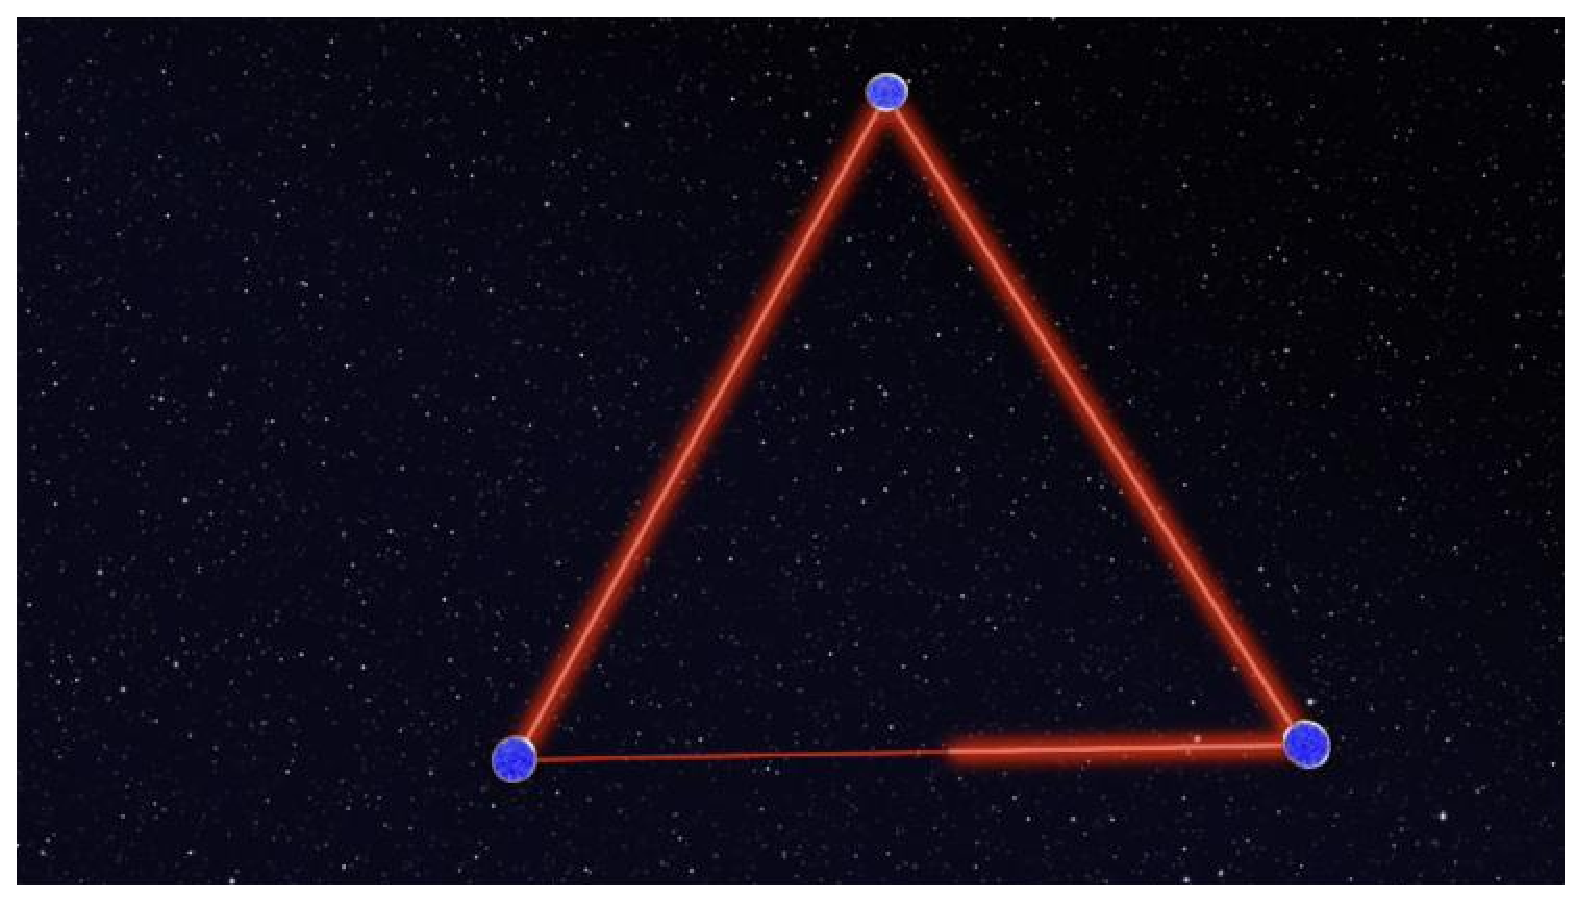
\includegraphics{eLISA}
\end{figure}

\begin{figure}
  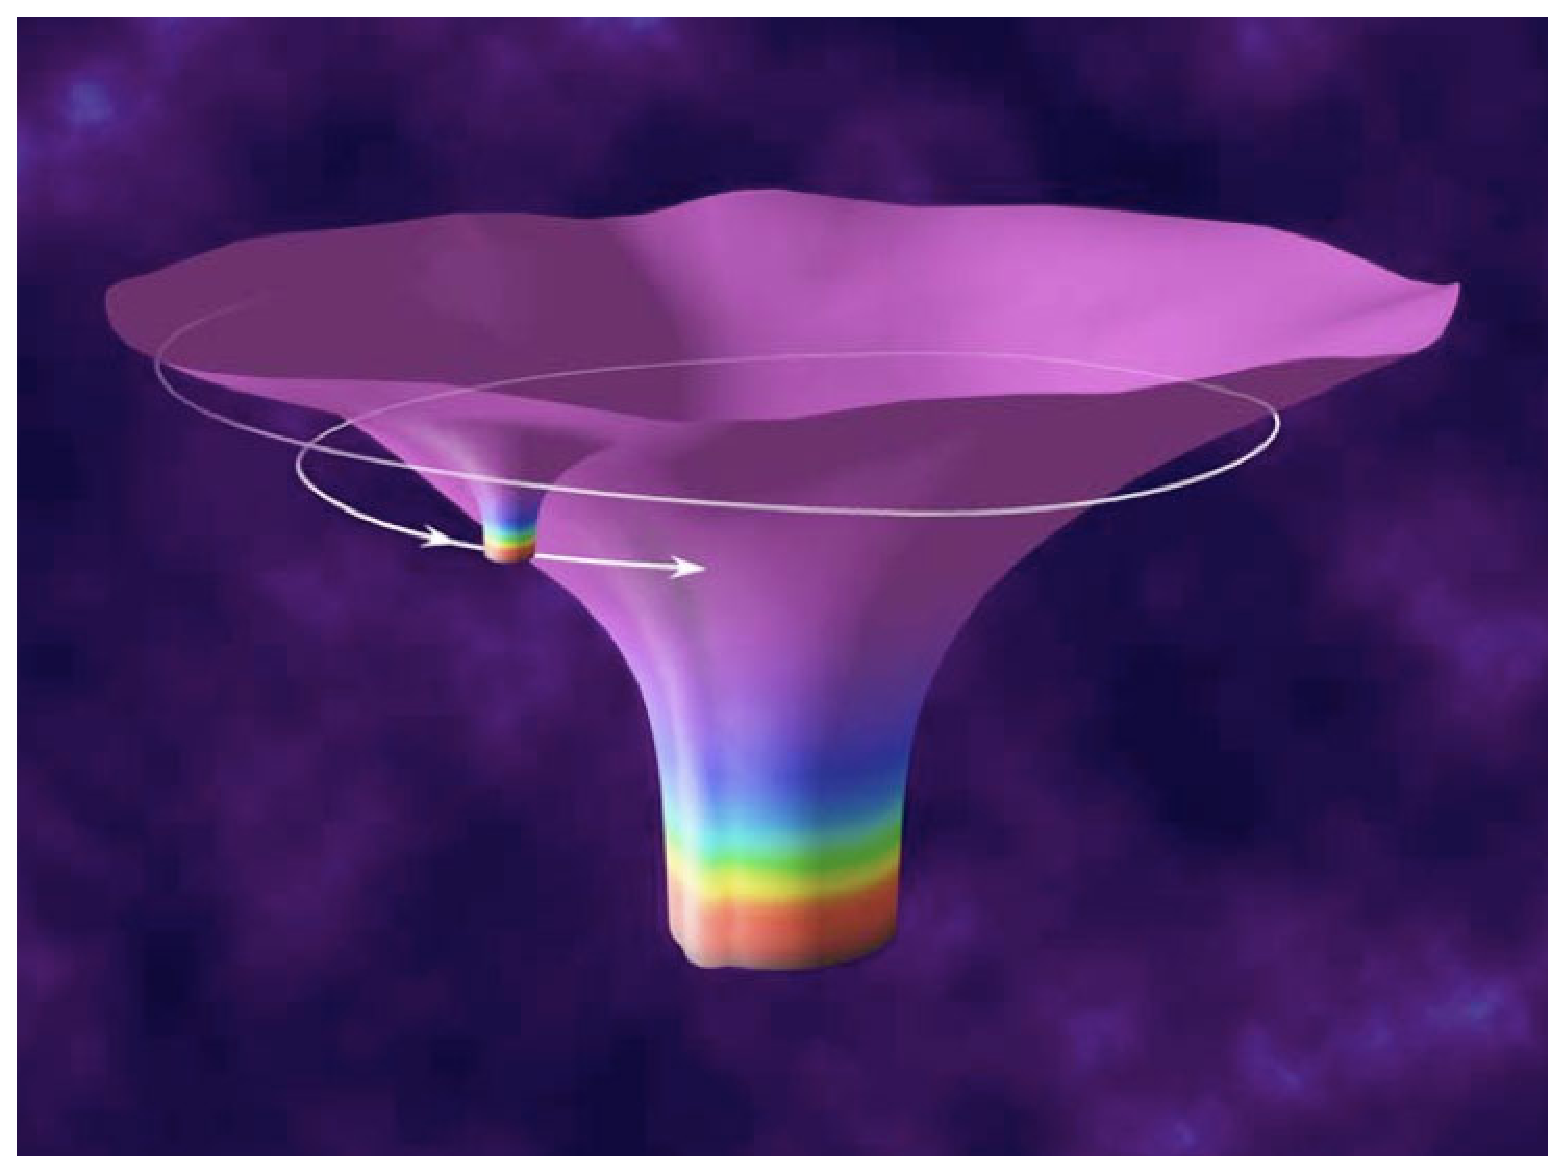
\includegraphics{EMRI}
\end{figure}



%Thornberg
%Warburton
%Wardell
%Diener
%adam pound
%bernard whiting
%ian vega
%anna hesthaven
%maarten van de meent
%jonathan thompson
%jordan moxon?

\section{Extreme Mass Ratio Inspirals}

\section{EMRIs}
\section{The discontinuous galerkin method}
\section{LISA}
